
\begin{appendices}
	
	\section{Two neurons neural network's cost}
	\label{sec:2N_NN_cost}
		Here we want to derive the cost $C$ of neural network\ref{fig:2N_NN} with respect to $x$. We first detail all the variables and then proceed to derivation.
		\begin{itemize}
			\item $C$ is the cost defined for sample $i$ as $C_i = y_i \ln(p_i) + (1-y_i)\ln(1-p_i)$, and the total cost $C$ is the mean of over the samples' costs.
			\item $p_i$ is the prediction for sample $i$. It's defined by $p_i = \sigma(z)$
			\item $\sigma(z)$ is the sigmoid function: $\sigma(z) = \frac{1}{1 + e^{-z}}$. It's derivative with respect to $z$ is $\sigma(z)(1-\sigma(z))$
			\item $z$ is a term introduced to narrow the notation. $z=W^Tx+b$.
			\item $W^T$ is the weight matrix such that $W^j$ is the weight vector for neuron $j$
			\item $b$ is a bias term. It can be considered as a weight to a feature always equal to one.
			\item $x_i$ is an input sample vector defined by its features.
		\end{itemize}
		Now, we use the chain rule to derive the Cost $C_i$ with respect to input $x$
		\begin{equation}
			\begin{split}
				\frac{\delta C_i}{\delta x} &= \frac{\delta C_i}{\delta p_i} \frac{\delta p_i}{\delta x} \\
				&= y_i \frac{1}{p_i} \frac{\delta p_i}{\delta x} + (1-y_i)\frac{1}{1-p_i} \frac{\delta (1-p_i)}{\delta x} \\
				&= \frac{y_i}{p_i} p_i(1-p_i)\frac{\delta z}{\delta x} + \frac{1-y_i}{1-p_i} -(p_i)(1-p_i) \frac{\delta z}{\delta x} \\
				&= \left( y_i (1-p_i) + (1-y_i) (-p_i)   \right) \frac{\delta z}{\delta x} \\
				&= W \left( y_i (1-p_i) + (1-y_i) (0-p_i)  \right)  \\
				&= W \left( y_i -p_i                       \right)
			\end{split}
		\end{equation}



	\section{Weight initialisation on simple example} % (fold)
	\label{sec:weight_initialisation_on_simple_example}

		The \fref{fig:simple_NN_init} shows our simple example initalized with some specific hand-engineered features.
		\begin{figure}[H]
			\centering
			\def\layersep{8em}	
			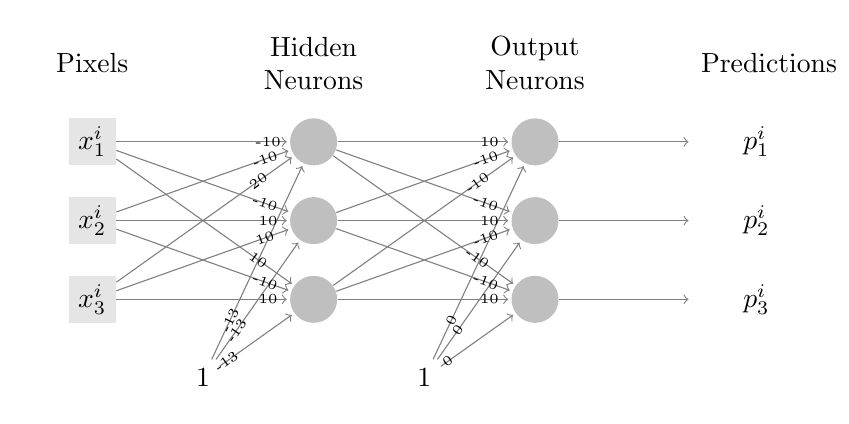
\begin{tikzpicture}[shorten >=1pt,->,draw=black!50, node distance=\layersep]
			    \tikzstyle{every pin edge}=[<-,shorten <=1pt]
			    \tikzstyle{pixel} = [rectangle, fill=black!10,minimum size=17pt,inner sep=0pt]
			    \tikzstyle{neuron}=[circle,fill=black!25,minimum size=17pt,inner sep=0pt]
			    \tikzstyle{annot} = [text width=4em, text centered]
			    \tikzstyle{annot2} = [text width=2em, text centered]
			    
			    %%% DRAW THE NODES
			    \foreach \name / \y in {1,2,3}
			        \node[pixel] (I-\name) at (0,-\y) {$x^i_\y$};
			    \node (I-4) at (\layersep*.5,-4) {$1$};

			    \foreach \name / \y in {1,...,3}
					\node[neuron] (H-\y) at (\layersep*1,-\y) {};
				\node (H-4) at (\layersep*1.5,-4) {$1$};
				
				\foreach \name / \y in {1,...,3}	
					\node[neuron] (O-\y) at (\layersep*2,-\y) {};
				
				\foreach \name / \y in {1,...,3}
					\node[annot] (P-\y) at (\layersep*3,-\y) {$p^i_\y$};

			    %%% DRAW THE PATHS
	            \path[every node/.style={sloped,anchor=west}] (I-1) edge node[annot]  {\tiny  -10 } (H-1);
	            \path[every node/.style={sloped,anchor=west}] (I-2) edge node[annot]  {\tiny  -10 } (H-1);
	            \path[every node/.style={sloped,anchor=west}] (I-3) edge node[annot]  {\tiny   20 } (H-1);
	            \path[every node/.style={sloped,anchor=east}] (I-4) edge node[annot]  {\tiny  -13 } (H-1);
	            \path[every node/.style={sloped,anchor=west}] (I-1) edge node[annot]  {\tiny  -10 } (H-2);
	            \path[every node/.style={sloped,anchor=west}] (I-2) edge node[annot]  {\tiny   10 } (H-2);
	            \path[every node/.style={sloped,anchor=west}] (I-3) edge node[annot]  {\tiny   10 } (H-2);
	            \path[every node/.style={sloped,anchor=east}] (I-4) edge node[annot2] {\tiny  -13 } (H-2);
	            \path[every node/.style={sloped,anchor=west}] (I-1) edge node[annot]  {\tiny   10 } (H-3);
	            \path[every node/.style={sloped,anchor=west}] (I-2) edge node[annot]  {\tiny  -10 } (H-3);
	            \path[every node/.style={sloped,anchor=west}] (I-3) edge node[annot]  {\tiny   10 } (H-3);
	            \path[every node/.style={sloped,anchor=east}] (I-4) edge node[annot2] {\tiny  -13 } (H-3);

	            \path[every node/.style={sloped,anchor=west}] (H-1) edge node[annot]  {\tiny   10 } (O-1);
	            \path[every node/.style={sloped,anchor=west}] (H-2) edge node[annot]  {\tiny  -10 } (O-1);
	            \path[every node/.style={sloped,anchor=west}] (H-3) edge node[annot]  {\tiny  -10 } (O-1);
	            \path[every node/.style={sloped,anchor=east}] (H-4) edge node[annot]  {\tiny    0 } (O-1);
	            \path[every node/.style={sloped,anchor=west}] (H-1) edge node[annot]  {\tiny  -10 } (O-2);
	            \path[every node/.style={sloped,anchor=west}] (H-2) edge node[annot]  {\tiny   10 } (O-2);
	            \path[every node/.style={sloped,anchor=west}] (H-3) edge node[annot]  {\tiny  -10 } (O-2);
	            \path[every node/.style={sloped,anchor=east}] (H-4) edge node[annot2] {\tiny    0 } (O-2);
	            \path[every node/.style={sloped,anchor=west}] (H-1) edge node[annot]  {\tiny  -10 } (O-3);
	            \path[every node/.style={sloped,anchor=west}] (H-2) edge node[annot]  {\tiny  -10 } (O-3);
	            \path[every node/.style={sloped,anchor=west}] (H-3) edge node[annot]  {\tiny   10 } (O-3);
	            \path[every node/.style={sloped,anchor=east}] (H-4) edge node[annot2] {\tiny    0 } (O-3);


			    \foreach \source in {1,...,3}
			            \path (O-\source) edge (P-\source);

			    %%% ANOTATE
			    \node[annot,above of=I-1, node distance=1cm] (iv) {Pixels};
			    \node[annot,above of=H-1, node distance=1cm] () {Hidden Neurons};
			    \node[annot,above of=O-1, node distance=1cm] () {Output Neurons};
			    \node[annot,above of=P-1, node distance=1cm] () {Predictions};

			\end{tikzpicture}
			\label{fig:simple_NN_init}
			\caption{Simple example with weight initialization}
		\end{figure}
	

	\section{Softmax layer}
	\label{sec:softmax_layer}
		tata
		


	\section{Vectors and matrices}
	\label{sec:vectors_and_matrices}
		\begin{itemize}
			\item $x^i$ is a vector. In the case of an image, it has as many values as there is pixels.
			\item $w^l$ is a matrix where each colums represent a feature detector. $w^l$ has as many columns as there is neurons on the layer $l$ and as many lines as there is inputs in layer $l-1$. On the \fref{fig:simple_NN_init} the weights correspond to the numbers initilized on the edges in between each layers.
			\item $b^l$ is a vector. It has as many values as there is neurons on the layer $l$.
		\end{itemize}
	




\end{appendices}
		

